%\documentclass[iop]{emulateapj}
%\documentclass[12pt, preprint]{emulateapj}
\documentclass[12pt, onecolumn]{emulateapj}

\usepackage{amsmath}
%\usepackage{bibtex}
%\bibliographystyle{unsrtnat}

\usepackage{tikz}
\usetikzlibrary{shapes.geometric, arrows}
\usetikzlibrary{fit}

\tikzstyle{hyper} = [circle, text centered, draw=black]%, fill=blue!30]
\tikzstyle{param} = [circle, text centered, draw=black]%, fill=green!30]
\tikzstyle{data} = [circle, text centered, draw=black, line width=2pt]%, fill=red!30]
%\tikzstyle{hyper} = [trapezium, trapezium left angle=70, trapezium right angle=110, minimum width=1cm, minimum height=0.5cm, text centered, draw=black, fill=green!30]
%\tikzstyle{param} = [rectangle, minimum width=1cm, minimum height=0.5cm, text centered, draw=black, fill=green!30]
%\tikzstyle{data} = [diamond, minimum width=1cm, minimum height=1cm, text centered, draw=black, fill=red!30]
%\tikzstyle{eqn} = [rectangle, minimum width=1cm, minimum height=0.5cm, text centered, draw=black]%, fill=green!30]
%\tikzstyle{latent} = [diamond, minimum width=1cm, minimum height=0.5cm, text centered, draw=black]%, fill=green!30]
\tikzstyle{arrow} = [thick,->,>=stealth]

\newcommand{\myemail}{aimalz@nyu.edu}
\newcommand{\textul}{\underline}

%\slugcomment{}

\shorttitle{Fully Probabilistic Ideas for HETDEX}
\shortauthors{Malz}

\begin{document}

\title{Fully Probabilistic Ideas for HETDEX}

\author{A.I. Malz\altaffilmark{1}}
\altaffiltext{1}{CCPP}
\email{aimalz@nyu.edu}

\begin{abstract}
This note covers some extensions of my work on cosmological inference with photo-z posteriors to applications within HETDEX.
\end{abstract}

\keywords{HETDEX}

\section{The problem}
\label{sec:intro}

This note concerns the OII emitter contamination of LAE galaxies in the HETDEX sample.  HETDEX aims to calculate the spatial correlation function of LAE galaxies at redshifts $1.5 \lesssim z \lesssim 2.5$.  Using IFU spectroscopy, HETDEX must identify these single emission line galaxies using other, much fainter emission and absorption lines.  At certain redshifts, the corroborating lines may not fall into the wavelength range over which HETDEX observes, leading to only a line indicating detection of some single emission line galaxy.  OII emitters are another single emission line galaxy type found at low redshifts $z \sim 0.2$ whose single emission line may be confused with that of Ly $\alpha$ when its corroborating lines also fall outside the wavelength range over which HETDEX observes.  Based on their emission lines alone, some LAEs and OIIEs thus cannot be distinguished, and the OIIEs are considered the predominant contaminating population of the HETDEX LAE sample.  

It is desirable to classify all $N$ single emission line galaxies in the HETDEX sample as type $T_{n}$ for the two options of $T^{LAE}$ and $T^{OII}$.  By considering photometrically determined equivalent width measurements $\{w_{n}\}_{N}$ in addition to the spectra $\{\vec{s}_{n}\}_{N}$, posterior probabilities $\{p(T_{n}|w_{n},\vec{s}_{n})\}_{N}$ may be constructed.  (See Leung, et al. 2016.)  A cut in posterior probability of $T^{LAE}$ may be made to construct the catalog used for the spatial correlation function.  

\section{A proposed solution}
\label{sec:confrac}

As an alternative, the set of posterior probabilities $\{p(T_{n}|EW_{n},\vec{s}_{n})\}_{N}$ may be used in full to calculate the posterior probability distribution of the contamination fraction $f$.  First, we introduce the probabilistic graphical model in Fig. \ref{fig:fT}.  There are two galaxy types $T$ to consider, that of $T^{LAE}$ and that of $T^{OII}$.  We wish to marginalize over these parameters $\{T_{n}\}_{N}$ to infer the contamination fraction $f$, a ratio of $N_{OII}$ and $N_{LAE}$.  We may without loss of generality also think of the function $f$ as the pair $N_{OII}$ and $N_{LAE}$.  The data $\vec{d}_{n}$ used to determine each posterior probability $p(T_{n}|\vec{d}_{n})$ of an individual galaxy's type given its data is comprised of its spectrum $\vec{s}_{n}$ and its photometrically-determined equivalent width $w_{n}$.

\begin{figure}
\vspace{0.5cm}
\begin{center}
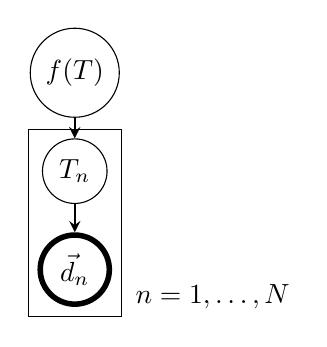
\begin{tikzpicture}[node distance=1cm]

\node (fT) [hyper] {$f(T)$};
\node (T) [param, below of=fT,yshift=-0.25cm] {$T_{n}$};
\node (specew) [data, below of=T,yshift=-0.25cm] {$\vec{d}_{n}$};
\node (survey) [draw=black,fit={(specew.west)(T.north)(specew.south)(specew.east)}] {};
\node [xshift=1.75cm,yshift=0.25cm] at (survey.south) {$n=1,\dots,N$};

\draw [arrow] (fT) -- (T);
\draw [arrow] (T) -- (specew);

\end{tikzpicture}
\caption{}
\label{fig:fT}
\end{center}
\end{figure}

The model of Fig. \ref{fig:fT} corresponds to the following equations for the posterior probability distribution $p(f|\{\vec{d}_{n}\}_{N})$.  

\begin{align*}
p(f|\{\vec{d}_{n}\}_{N}) &= p(\{\vec{d}_{n}\}_{N}|f)\frac{p(f)}{p(\{\vec{d}_{n}\}_{N})}\\
&\propto p(\{\vec{d}_{n}\}_{N}|f)p(f)\\
&\propto p(f)\prod_{n=1}^{N}p(\vec{d}_{n}|f)\\
&\propto p(f)\prod_{n=1}^{N}\int p(\vec{d}_{n}|T_{n})p(T_{n}|f)dT_{n}\\
&\propto p(f)\prod_{n=1}^{N}\int p(\vec{d}_{n}|T_{n})p(T_{n}|f)\frac{p(T_{n}|\vec{d}_{n},f^{0})}{p(T_{n}|\vec{d}_{n},f^{0})}dT_{n}\\
&\propto p(f)\prod_{n=1}^{N}\int p(T_{n}|f)p(\vec{d}_{n}|T_{n})p(T_{n}|\vec{d}_{n},f^{0})\frac{p(\vec{d}_{n}|f^{0})}{p(\vec{d}_{n}|T_{n},f^{0})p(T_{n}|f^{0})}dT_{n}\\
&\propto p(f)\prod_{n=1}^{N}\int p(T_{n}|\vec{d}_{n},f^{0})\frac{p(\vec{d}_{n}|T_{n})p(\vec{d}_{n}|f^{0})}{p(\vec{d}_{n}|T_{n},f^{0})}\frac{p(T_{n}|f)}{p(T_{n}|f^{0})}dT_{n}\\
&\propto p(f)\prod_{n=1}^{N}\int p(T_{n}|\vec{d}_{n},f^{0})\frac{p(T_{n}|f)}{p(T_{n}|f^{0})}dT_{n}
\end{align*}

The code produced by Malz \& Hogg 2016 can be run to sample this posterior distribution over the contamination fraction parameter, as the problem is essentially that of a two-bin histogram representation of $N(T)$.   

\section{Toy Model}
\label{sec:toy}

We may also consider the simpler case of a survey in which all galaxies have one of exactly two redshifts sufficiently apart that one would expect no correlation between the power spectra at each redshift.  In the case in which we are interested solely in one group and not in the other, hereafter referred to as the contaminating population, we wish to estimate the power spectrum of that group given some incompleteness and contamination.  In this case, the three dimensional galaxy map is a linear combination of galaxies from each of the two populations, and since the two possible redshifts are distant from one another, the power spectrum of the combined sample will be a linear combination of the power spectra of each individual population.  In this problem, several questions can be investigated.

\begin{itemize}
\item Can we analytically solve for the power spectrum of the population of interest in terms of the observed power spectrum and contamination/incompleteness fractions?
\item Can the observed power spectrum of the two groups be used to identify misclassified galaxies and reclassify their redshifts in an iterative calculation of the power spectrum?
\item If instead of deterministic redshift assignments we have probabilities for each galaxy, can they be used to infer the posterior of the power spectrum of interest?
\end{itemize}

This problem is also similar to that of blended objects, in which we observe more than one galaxy but classify it as a single galaxy due to the close proximity on the sky of the galaxies in question.  Redshift estimation in this case can be catastrophically wrong, but discrimination of blended systems could be valuable in improving the power spectrum calculated from the blended galaxy map.  Again, in this toy model, it would be of interest to investigate how the observed power spectrum is affected by blended objects and whether it can be corrected through an iterative procedure on the identification of blended systems.

%\section{Power Spectrum}
%\label{sec:powspec}

%\acknowledgments

%\appendix

\bibliography{references}

\end{document}